\documentclass[12pt,letterpaper]{article}
\usepackage[utf8]{inputenc}
\usepackage[spanish]{babel}
\usepackage{graphicx}
\usepackage[left=2cm,right=2cm,top=2cm,bottom=2cm]{geometry}
\usepackage{graphicx} % figuras
% \usepackage{subfigure} % subfiguras
\usepackage{float} % para usar [H]
\usepackage{amsmath}
%\usepackage{txfonts}
\usepackage{stackrel} 
\usepackage{multirow}
\usepackage{enumerate} % enumerados
\renewcommand{\labelitemi}{$-$}
\renewcommand{\labelitemii}{$\cdot$}
% \author{}
% \title{Caratula}
\begin{document}

% Fancy Header and Footer
% \usepackage{fancyhdr}
% \pagestyle{fancy}
% \cfoot{}
% \rfoot{\thepage}
%

% \usepackage[hidelinks]{hyperref} % CREA HYPERVINCULOS EN INDICE

% \author{}
\title{Caratula}

\begin{titlepage}
\begin{center}
\large{UNERSIDAD PRIVADA DE TACNA}\\
\vspace*{-0.025in}
\begin{figure}[htb]
\begin{center}

\includegraphics[width=8cm]{./Imagenes/logo}
\end{center}
\end{figure}
\vspace*{0.15in}
INGENIERIA DE SISTEMAS  \\

\vspace*{0.5in}
\begin{large}
TITULO:\\
\end{large}

\vspace*{0.1in}
\begin{Large}
\textbf{INFORME DE LABORATORIO No 02} \\
\end{Large}

\vspace*{0.3in}
\begin{Large}
\textbf{CURSO:} \\
\end{Large}

\vspace*{0.1in}
\begin{large}
BASE DE DATOS II\\
\end{large}

\vspace*{0.3in}
\begin{Large}
\textbf{DOCENTE(ING):} \\
\end{Large}

\vspace*{0.1in}
\begin{large}
 Patrick Cuadros Quiroga\\
\end{large}

\vspace*{0.2in}
\vspace*{0.1in}
\begin{large}
Integrantes: \\
\begin{flushleft}
Renzo	A. Moreno Cáceres	           \hfill	(2013047246) \\
Mamani Limache, Jhony 		\hfill	(2013046566) \\
Ordoñez Quilli, Ronald         	\hfill	(2015052821)   \\
Zavala Venegas, Luis Angel         \hfill	(2010037899) \\
Nombre Estudiante No 5       	\hfill	(Codigo 05) \\
\end{flushleft}
\end{large}
\end{center}

\end{titlepage}


\tableofcontents % INDICE
\thispagestyle{empty} % INDICE SIN NUMERO
\newpage
\setcounter{page}{1} % REINICIAR CONTADOR DE PAGINAS DESPUES DEL INDICE

\section{Actividad No 01 – Manipulaci\'on de Datos} 

\begin{enumerate}[1.]
	\item El departamento de Recursos Humanos requiere crear sentencias SQL para insertar, actualizar y eliminar datos de empleados. Como prueba se utilizará la tabla Mis\_Empleados antes de remitir las sentencias al departamento de Recursos Humanos.

	\item Crear la tabla Mis\_Empleados utilizando la siguiente estructura.
	\begin{center}
	\includegraphics[width=5cm]{./Imagenes/imagen0102} 
	\end{center}
	\begin{center}
	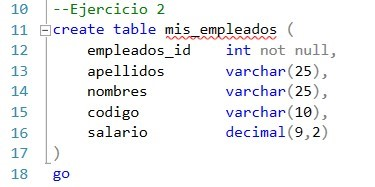
\includegraphics[width=8cm]{./Imagenes/img2} 
	\end{center}
	\item Generar una sentencia de inserción de datos que permita añadir los siguientes registros:
	\\
	\\ insert into mis\_empleados values (1, 'Vargas Canseco','Raúl', 'rvargas', 895),(2, 'Castro Feria',  'María','mcastro', 860);
	\\ go

	\begin{center}
	\includegraphics[width=8cm]{./Imagenes/imagen0103} 
	\end{center}
	\begin{center}
	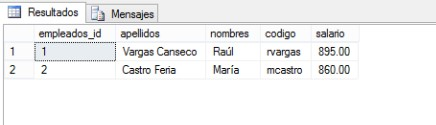
\includegraphics[width=12cm]{./Imagenes/img3} 
	\end{center}
	\item Generar un script que permita que mediante utilización de variables de sustitución, la inserción de información en la tabla Mis\_Empleados.
	\begin{center}
	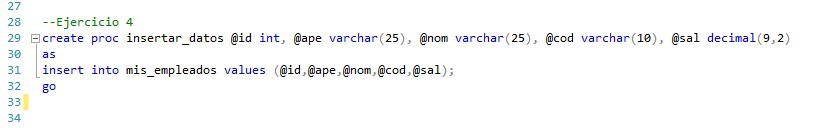
\includegraphics[width=18cm]{./Imagenes/img4} 
	\end{center}
	\item Utilizando el script anterior adicionar los siguientes registros.
	\begin{center}
	\includegraphics[width=5cm]{./Imagenes/imagen0105} 
	\end{center}
	\begin{center}
	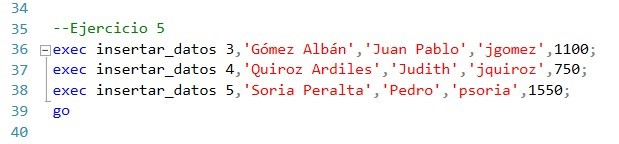
\includegraphics[width=18cm]{./Imagenes/img5} 
	\end{center}
	\item Revisar los cambios hechos a la tabla.
	\\
	\\ select * from mis\_empleados
	\\ go
	
	\begin{center}
	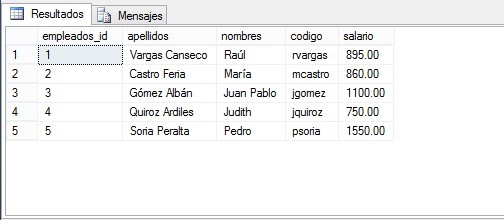
\includegraphics[width=10cm]{./Imagenes/img6} 
	\end{center}
	\item Cambiar el nombre del empleado No 3 a Benjamín.
	\\
	\\ update mis\_empleados set nombres='Benjamin' where empleados\_id=3;
	\\ go

	\begin{center}
	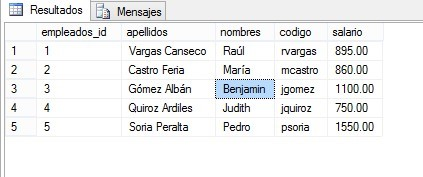
\includegraphics[width=10cm]{./Imagenes/img7} 
	\end{center}
	\item Elevar el salario a \$ 1,000 a todos los empleados que tengan un salario menor a esa cantidad.
	\\
	\\ update mis\_empleados set salario=1000 where salario<1000;
	\\ go

	\begin{center}
	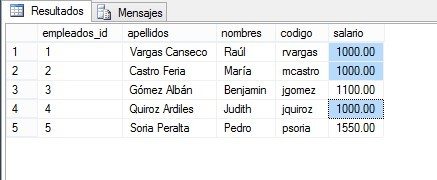
\includegraphics[width=10cm]{./Imagenes/img8} 
	\end{center}
	\item Eliminar el registro del empleado María Castro
	\\
	\\ delete from mis\_empleados where codigo='mcastro';
	\\ go

	\begin{center}
	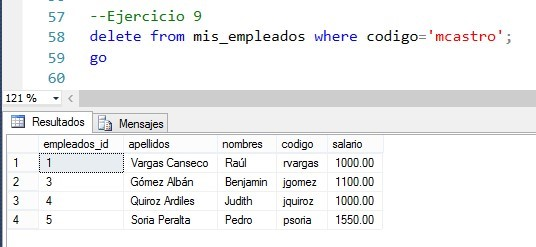
\includegraphics[width=10cm]{./Imagenes/img9} 
	\end{center}
	\item Revisar los cambios hechos a la tabla.
	\\
	\\ select [Begin Time],[RowLog Contents 1],[Transaction Name],Operation 
	\\from sys.fn\_dblog(NULL,NULL) 
	\\where AllocUnitName='dbo.mis\_empleados' and Operation IN ('LOP\_DELETE\_ROWS')
	\\ go

	\begin{center}
	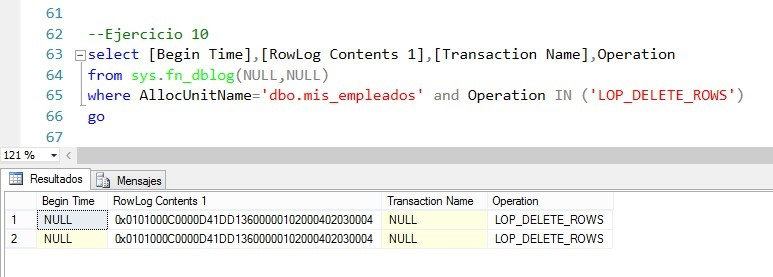
\includegraphics[width=10cm]{./Imagenes/img10} 
	\end{center}
	\item Confirmar los cambios a la tabla.
	\\
	\\ select * from mis\_empleados
	\\ go

	\begin{center}
	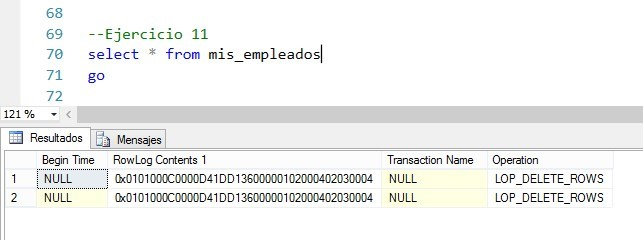
\includegraphics[width=10cm]{./Imagenes/img11} 
	\end{center}
	\item Adicionar el siguiente registro a la tabla
	\item Revisar la adición realizada
	\item Crear un punto de restauración intermedio para esta transacción
	\item Borrar los registros de la tabla MIS\_EMPLEADOS.
	\item Revisar los cambios realizados.
	\item Descartar los cambios hechos a la tabla sin descartar la última adición hecha.
	\item Revisar nuevamente los registros de la tabla MIS\_EMPLEADOS.
	\item Confirmar todos los cambios hechos a la tabla MIS\_EMPLEADOS.
	\item Modificar el script del punto 4.4. a fin de que se genere automáticamente el CODIGO del empleado que lo conforman la primera letra de su nombre y la primera palabra de su apellido.
	\item Adicionar el siguiente registro a la tabla a fin de corroborar el funcionamiento del script anterior
	\item Revisar los cambios realizados. Y finalmente confirmar todos los cambios hechos a la tabla MIS\_EMPLEADOS.

\end{enumerate} 


\section{Actividad No 02 – Reconociendo la estructura} 

\begin{enumerate}[1.]
	\item Crear la tabla Departamentos utilizando la siguiente estructura:
	\\
           \\create table Departamentos (
		\\ID int not null,
		\\nombre varchar (25))
		\\go
	\begin{center}
	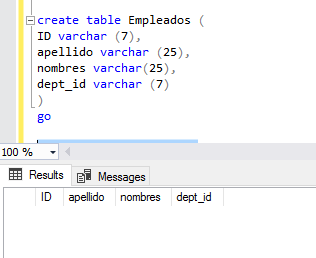
\includegraphics[width=10cm]{./Imagenes/prac2eje1} 
	\end{center}
	\item Poblar la tabla Departamentos con los datos de la tabla Departments.
	\\
		\\create table Empleados (
		\\ID varchar (7),
		\\apellido varchar (25),
		\\nombres varchar(25),
		\\dept\_id varchar (7))
		\\go
	\begin{center}
	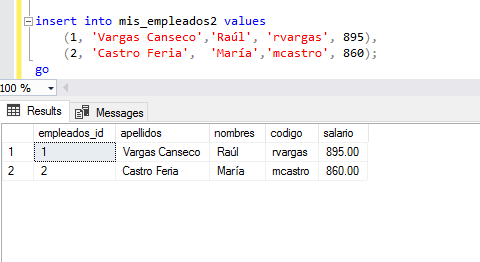
\includegraphics[width=10cm]{./Imagenes/prac2eje2} 
	\end{center}
	\item Crear la tabla Empleados utilizando la siguiente estructura.
	\\
	\\create table mis\_empleados2(
	\\empleados\_id	int not null,
	\\apellidos		varchar(25),
	\\nombres			varchar(25),
	\\codigo			varchar(10),
	\\salario			decimal(9,2))
	\\go
	\begin{center}
	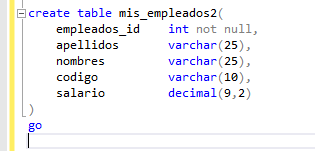
\includegraphics[width=10cm]{./Imagenes/prac2eje3} 
	\end{center}
	\item Crear la tabla Empleados2 basada en la estructura de la tabla Employees. Incluir solo las columnas EMPLOYEE\_ID, FIRST\_NAME, LAST\_NAME, SALARY y DEPARMENT\_ID 		respectivamente.
	\\
	\\create table mis\_empleados3(
	\\empleados\_id	int not null,
	\\apellidos		varchar(25),
	\\nombres			varchar(25),
	\\codigo			varchar(10),
	\\salario			decimal(9,2))
	\\go
	\begin{center}
	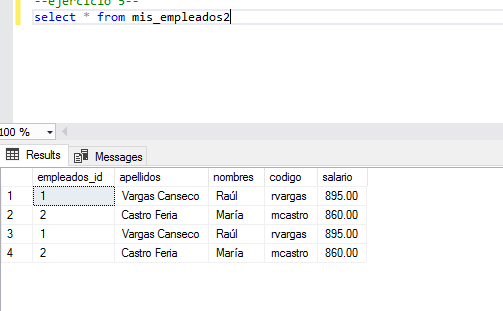
\includegraphics[width=10cm]{./Imagenes/prac2eje5} 
	\end{center}
	\item Modificar el estado de la tabla Empleados2 a SOLO LECTURA.
	\item Tratar de adicionar el siguiente registro a la tabla Empleados2.
	\\
	\\insert into mis\_empleados2 values
	\\(1, 'Vargas Canseco','Ra\'ul', 'rvargas', 895),
	\\(2, 'Castro Feria',  'Mar\'ia','mcastro', 860);
	\\go
	\item Revertir el estado de la tabla LECTURA / ESCRITURA. Tratar de insertar nuevamente la información del punto 4.6.
	\item Eliminar la tabla Empleados2.
	\\
	\\drop table mis\_empleados2
	\begin{center}
	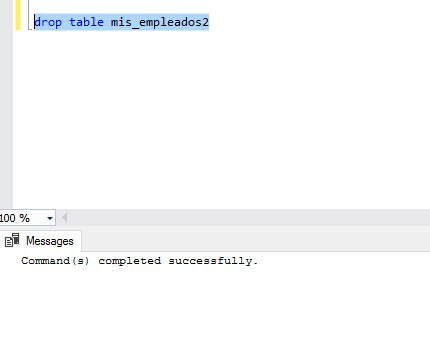
\includegraphics[width=10cm]{./Imagenes/prac2eje8} 
	\end{center}
	
\end{enumerate}
\section{Actividad No 03 –  Otros objetos de base de datos} 
		
\begin{enumerate}[1.]
	\item El Departamento de Recursos Humanos requiere ocultar ciertos datos de la tabla EMPLOYEES, Ellos necesitan una vista llamada VW\_Empleados, que contenga los campos ID del Empleado, Nombres e ID del Departamento.
	\item Utilizando la vista anterior crear un reporte que muestre los nombres y departamentos a los cuales
pertenecen los empleados.
	\item El departamento 50 requiere acceso a los datos de los empleados. Generar una vista llamada VW\_Dept50, que contenga las columnas ID del Empleado, Apellidos e ID del Departamento de los empleados del departamento 50. Etiquetar las columnas como EmpNo, Empleado y DeptNo. Por razones de seguridad no se debe permitir a los empleados ser reasignados a otros departamentos.
	\item Probar la vista, tratando de reasignar al empleado Matos al departamento 80.

	

	\item Se requiere crear una secuencia que será utilizada en la Llave Primaria de la tabla Departamentos (tabla creada en la práctica anterior). La secuencia deberá iniciar con el valor 200 y terminar en el valor 1000, asimismo deberá incrementarse en 10 cada vez que se requiera. Nombrar la secuencia SEQ\_Departamentos\_ID.
	\\ \\ create sequence SEQ\_Departamentos\_ID start with 200 increment by 10 maxvalue 1000 minvalue 200;	
	
	\begin{center}
	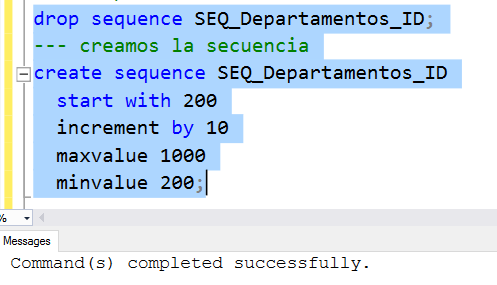
\includegraphics[width=5cm]{./Imagenes/actividad_03_05} 
	\end{center}

	\item Para probar la secuencia, adicionar dos registros a la tabla Departamentos, Educación y Administración. Verificar la adición.
	\\ \\ declare @liCodigo int select @liCodigo = next value for SEQ\_Departamentos\_ID insert into departments  values(@liCodigo,'matematica','300','3300') select * from departments

	\begin{center}
	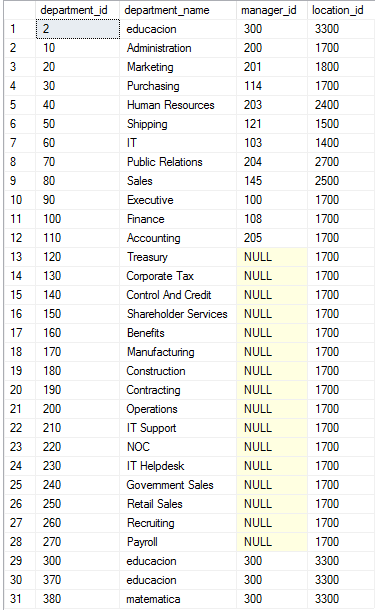
\includegraphics[width=5cm]{./Imagenes/actividad_03_06} 
	\end{center}

	\item Crear un índice no único en la columna NOMBRE de la tabla Departamentos.
	\\ \\CREATE INDEX Indice\_no\_unico ON departments (department\_name);

	\begin{center}
	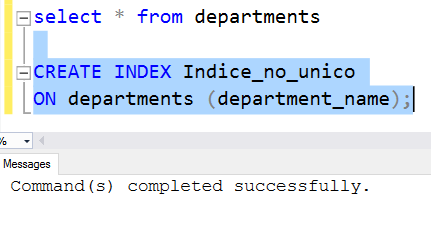
\includegraphics[width=5cm]{./Imagenes/actividad_03_07} 
	\end{center}	

	\item Crear un sinónimo para la tabla EMPLOYEES con el nombre EMP.
	\\ \\EXECUTE sp\_addlinkedserver Server1;  GO CREATE SYNONYM EMP FOR Server1.AdventureWorks2012.HumanResources.Employee; GO 	

	\begin{center}
	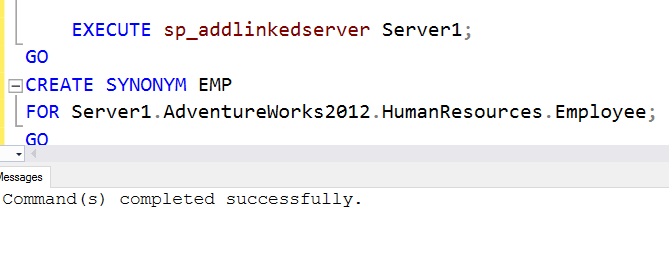
\includegraphics[width=5cm]{./Imagenes/actividad_03_08}  
	\end{center}	

\end{enumerate}



\end{document}
